\documentclass[10pt,letterpaper]{article}
\usepackage[margin=1in]{geometry}
\usepackage[T1]{fontenc}
\usepackage{lmodern,microtype,amsmath,amssymb,amsthm,booktabs,array,graphicx,xurl,longtable}
\usepackage[hidelinks]{hyperref}
\microtypesetup{protrusion=false}
\setlength{\parskip}{3pt}
\setlength{\parindent}{1em}
\newtheorem{proposition}{Proposition}
\newtheorem{lemma}[proposition]{Lemma}
\newcommand{\ind}{\mathbf 1}
\newcommand{\dist}{\operatorname{dist}}
\title{Supplement: Certified Expression Intervals\\under Shared Segmentation Uncertainty}
\author{Arnav Peram}\date{}
\hypersetup{pdftitle={Supplement: Certified Expression Intervals under Shared Segmentation Uncertainty},pdfauthor={Arnav Peram}}
\begin{document}\maketitle
This supplement specifies the atlas construction, exact count algorithm, experimental contracts and verification paths. The main manuscript contains the complete cost-representation, gluing, hard-budget and composition arguments. All count guarantees concern the retained observed molecules and the declared fixed-seam family. The external breast input is explicitly a vendor format-test dataset, rather than biological validation.

\section{Physical atlas and exact reference agreement}
The reference is the original labelled raster interpreted as a union of closed pixel squares with disjoint interiors. A positive cell label is eligible when its pixel set is connected and does not meet the crop boundary. Background label zero may participate as the other side of an interface; it is not an additional biological cell. Ineligible cells, crop boundaries and unselected portions of interfaces remain fixed.

For each adjacent eligible label pair, trace shared pixel edges into paths. Split paths at vertices where continuation is ambiguous and into coordinate-monotone runs. Divide long runs at a maximum of 128 unit edges, trim one edge from each end, and retain at least four remaining edges. Rank candidates by length and then by a deterministic label/coordinate ordering. Try ribbon halfwidths $4,2,1,1/2$ pixels in that order. No gene identity, transcript count, count interval or optimization outcome determines this ranking.

Let $s_x,s_y\in\{-1,1\}$ orient a monotone run. Pixel-edge coordinates obey
\[
 t=s_xx+s_yy,\qquad u=s_xx-s_yy.
\]
The run is exactly $u=r(t)$, with slopes $+1$ or $-1$ between its recorded raster vertices. Put $v=u-r(t)$. The inverse physical chart, up to its stored origin, is
\[
 \Phi(t,v)=\frac p2\bigl(s_x(t+r(t)+v),\ s_y(t-r(t)-v)\bigr),
 \qquad |\det D\Phi|=\frac{p^2}{2}.
\]
The pixel size $p$ is read from the source coordinate transformation and represented rationally. It is not replaced by a rounded display value. An accepted ribbon has $v\in[-B,B]$, allowed displacement $|h(t)|\le3B/4$, $|h(t)-h(t')|\le|t-t'|$, and zero endpoint displacement. RNA clearance is $10^{-6}$ micrometres converted through the chart's transverse scale. These settings define a sensitivity family, not a fitted confidence region.

\subsection{Acceptance and nuclear constraints}
Every piece of the left/right half-ribbon is clipped against intersecting native pixels using rational polygon arithmetic. Positive-area intersections must have the declared left/right source labels. Pairwise ribbon interiors must be disjoint. A geometric spatial index reduces candidate comparisons; it does not replace the final rational intersection test. RNA coordinates are transformed through the exact chart and their nominal side must agree with the original source mask. A molecule may occur in at most one accepted patch.

A nuclear-mask pixel is labelled by the source \emph{cell} mask at that pixel, rather than by its unrelated nucleus identifier. Clip its square to the ribbon, transform its fragments into $(t,v)$ coordinates, and split at reference-curve knots. Over each projected interval, the maximum required left-side value or minimum right-side value supplies a conservative constant bound. Thus every original intersecting nuclear fragment retains its label. The bound may exclude additional shapes; it never permits a part of the nucleus to change owner. Structural constraints have zero additional clearance. Encoding them as shifted synthetic point/interval constraints cancels the engine's RNA clearance exactly; these encodings are not new RNA observations.

An initial nucleus-free extraction was retained as an unsuccessful coverage pilot. The final procedure keeps nuclear constraints and includes cell--background interfaces. This amendment preceded the new count calculations. It was fixed before the external transfer results. It is documented experimental ordering, not external preregistration.

\subsection{Global homeomorphism}
For fixed longitudinal coordinate and any admissible $h$, define
\[
 H_h(t,v)=\begin{cases}
 -B+(v+B)(h(t)+B)/B,&-B\le v\le0,\\
 h(t)+v(B-h(t))/B,&0\le v\le B.
 \end{cases}
\]
Its transverse slopes are strictly positive because $|h|<B$. Both formulas agree at zero, map zero to $h$, and fix $-B,B$. Its inverse is continuous, and $h=0$ at longitudinal endpoints makes the whole boundary trace fixed. Conjugating $(t,v)\mapsto(t,H_h(t,v))$ through $\Phi$ gives a homeomorphism of the closed physical ribbon fixing its boundary. It maps the two source sides to the requested alternatives.

Extend each map by the identity outside its ribbon. Disjoint interiors and fixed traces make the maps agree on intersections. A finite union is therefore a global continuous bijection with the corresponding piecewise inverse. The reference cell topology, connectivity, holes and junction incidences are preserved. This argument does not require deleting a complicated set of patches from a cell and hoping the remaining core is connected.

Changed-label area inside one two-label ribbon is exactly
\[
 A(h)=\frac{p^2}{2}\int_I |h(t)|\,dt.
\]
Interiors do not overlap, so changed-label area in the atlas is the sum of these costs, counted once. At source knots the chart is piecewise affine; the finite kink set has zero area. An arbitrary curved coordinate chart would require its own Jacobian and is not silently covered by this calculation.

\section{Exact assignment-cost function and graph construction}
In an ordered corridor, each boundary has a slope bound, band and endpoint values; adjacent boundaries have constant minimum and optional maximum separations. All finite rational data are binary encoded. The source satisfies the geometric constraints. RNA-location rectangles and pinned structural regions induce lower or upper interval requirements depending on their discrete owner thresholds.

The maximum-path closure $\Delta$ of same-coordinate separation inequalities yields
\[
 K_{ab}(r)=\max_c\{\Delta_{ac}+\Delta_{cb}-s_cr\}.
\]
Every finite sequence of permitted longitudinal and cross-boundary steps is bounded by such a term: choose the least slope on that path, bound its total travel below by the endpoint distance, and its remaining directed weights above by the corresponding closure weights. This gives the complete propagated lower/upper restrictions, including both directions of each finite maximum gap.

The selected lower family $L$, upper family $U$, and reference $f^0$ obey the same geometric difference inequalities. The finite conflict tests imply $L\le U$. Minimum and maximum preserve these inequalities and each scalar slope bound, so
\[
 f_b^*(t)=\min\{U_b(t),\max\{L_b(t),f_b^0(t)\}\}
\]
is a jointly feasible family and is pointwise nearest to the reference. This simultaneous attainment establishes the ownerwise minimum $D^*(c)$, not just a lower bound on independently chosen coordinates.

\subsection{Integrated layers and the helper bound}
In one direction, source-relative excursions are maxima of active flat-top cones. On an analytic interval with ordered positive heights $h_1\ge\cdots\ge h_q>0$, set $h_{q+1}=0$. Their activated maximum equals
\[
 \sum_{j=1}^{q}(h_j-h_{j+1})\,
 \ind[\text{at least one activation among the first }j\text{ occurs}].
\]
Integrate the affine differences exactly. Repeated cones carrying the same molecular bit use that bit once; complementary activations encode the opposite direction. Fixed-positive constraints contribute a mandatory constant or forced helper. Standard implication/OR gadgets then preserve the exact integral for every hard-feasible owner vector. Finite hard capacities exceed the total finite capacity for the requested objective.

For $M$ untruncated flat-top cones, a pair changes order only constantly many times. Starting with $M$ prefixes, each adjacent swap introduces at most one additional prefix. Thus the union contains $O(M^2+M)$ distinct sets. A common reference changes positivity, not cone order. Resolve simultaneous events into adjacent swaps and retain a deterministic tie rule on coincidence intervals. Mapping cone indices to repeated activation labels cannot enlarge the family. A set can use a predecessor prefix plus its last newly added label; retaining zero-weight predecessors keeps the arc count proportional to the number of sets.

If $M_b=O(Nm^2)$ includes all propagated molecular and structural constraints, the graph has
\[
 |V|=O\!\left(Gm+\sum_b(M_b^2+M_b)\right),\quad
 |E|=O\!\left(Gm+N^2m^2+\sum_b(M_b^2+M_b)\right).
\]
The auxiliary contribution is $O(N^2m^5)$. Source knots, intersections and coefficient denominator lengths still affect construction and encoding. Event-driven accumulation can integrate a direction's coefficients in $O((M^2+MJ+J+1)\log(M+J+2))$ rational-arithmetic and bitset operations for a $J$-knot reference. This integration-stage statement is distinct from the final graph-size bound and from total bit complexity. These inherited optional-optimization results are not retimed in the present atlas study.

\section{Critical-height count algorithm}
\subsection{Input contract and common mesh}
The implemented count chain accepts one boundary, fixed structural regions, rational piecewise-affine source, slope/band/endpoints, and one point per free RNA group. It rejects a free group spanning several locations or any non-point location box. Longitudinal intervals require owner memory across nodes; overlapping horizontal ownership thresholds can make ownership ambiguous at one height. These restrictions apply to raw inputs before mode-specific geometric transformations, including possible-outer mode. A regression test retains the overlapping-box counterexample that exposed the missing validation. Fixed groups may contain many structural rectangles because their labels are known. Group scores are nonnegative integers for each owner, with an integer fixed offset.

Collect all affine pieces that any canonical realization can select: lower and upper cones for every possible point owner, fixed constraints, bands, endpoints and source. Include all piece endpoints, observation locations and same-boundary intersections in a common mesh. Omit crossings outside the forced envelope only when they cannot be a canonical switch. At every node, candidate heights are function values inside the forced range and outside every observation's clearance gap.

For any complete feasible assignment, its canonical minimizer selects affine pieces between mesh events and crosses the source only at events. Its nodal trapezoidal area is exactly its continuous area. Conversely a feasible candidate path interpolates into a feasible boundary, and its trapezoid upper-bounds that interpolant's area. Retaining the canonical minimizer proves equality of minimum area at \emph{each count}, not equality for every interpolant.

\subsection{Recurrence, sliding minima and reconstruction}
Let $V_j$ be the sorted heights at time $t_j$, $z_j(v)$ the score of points observed at that time, and
\[
 a_j(v)=w_j|v-f^0(t_j)|,\qquad
 w_j=\tfrac12[(t_j-t_{j-1})+(t_{j+1}-t_j)],
\]
with missing endpoint intervals omitted. Each point contributes once. Pinned-group scores enter the initial offset. The least prefix cost satisfies
\[
 F_j(v,q)=a_j(v)+
 \min_{\substack{u\in V_{j-1}\\|u-v|\le s(t_j-t_{j-1})}}
 F_{j-1}(u,q-z_j(v)).
\]
Initialize with first-node cost and score. For each predecessor count, scan candidate heights in increasing order. Insert each permitted predecessor into a monotone deque, discard dominated costs at its back, and discard expired heights at its front. The front gives the least predecessor cost. Both ends of the height-compatibility interval move monotonically, so one node transition takes $O(H_{j-1}+H_j)$ work per count. Backpointers reconstruct a complete owner vector and boundary, which are checked against the original continuous constraints and exactly integrated area.

If the variable score range is $W$, dynamic-programming work is $O((W+1)\sum_jH_j)$ and full backpointer storage has the same order. Value-only rolling storage can be smaller. With $P$ explicit affine pieces, a conservative mesh bound is $O(P^2+P)$ events, at most $O(P)$ heights per event, and $O((W+1)P^3)$ dynamic-programming work. For explicit unit transcripts, $W$ is at most the number of scored molecules. Binary-compressed multiplicities instead give a pseudo-polynomial dependence on $W$. Rational operand lengths, candidate preparation and output serialization remain separate costs.

The implementation raises a resource-limit outcome instead of marking an incomplete spectrum exact. The reference is geometrically feasible but need not realize every point's original owner at zero cost. A positive mandatory-area test exercises that distinction. Single-copy source-feasible queries use the cheaper implication-closure fast path; all multicopy queries in the end-to-end count-chain census use the algorithm above.

\subsection{An explicit unit-molecule penalty gap}
Use source zero on $[0,30]$, slope one, band $[-4,4]$ and clearance $\rho=1/10$. At centers 5, 15 and 25 place respectively 2, 3 and 3 distinct point RNAs. Point $j$ in a cluster has $(t,x)=(\text{center}+j/100,\ h-j/100-\rho)$, with $h=2,3,3$. The slope and clearance force a common owner within each cluster; their leading tents dominate, and clusters have disjoint positive supports. Full owner enumeration gives eight feasible vectors and spectrum
\[
 \{(0,0),(2,4),(3,9),(5,13),(6,18),(8,22)\}
\]
(count, area). At area ten the largest attainable count is three. Every penalty bound is at least four: for $\mu\le1/3$ the count-eight state gives $8-12\mu\ge4$, and for $\mu\ge1/3$ the count-two state gives $2+6\mu\ge4$. At $1/3$ equality holds. All molecules are unit observations at distinct coordinates; no succinct bundle encoding is used. The count chain recovers the unsupported count-three outcome.

\section{Composition, baselines and joint predicates}
For a cell--gene pair with source count $n_0$, each incident patch supplies minimum physical area $S_i(d)$ for count \emph{change} $d$. Use
\[
 S(q)=\min_{d_1+\cdots+d_r=q}\sum_iS_i(d_i),\qquad
 [L,U]=\left[\min_{S(q)\le\delta}(n_0+q),\ 
 \max_{S(q)\le\delta}(n_0+q)\right].
\]
Using changes prevents counting fixed exterior molecules more than once. Zero-relevant patches can stay at their zero-cost source. A minimizing trace yields compatible local witnesses, and the global homeomorphism proves attainability. Restricting any allowed global state to its patches proves the reverse inequality. There is one budget for the complete atlas, not one independent allowance per patch.

The outer baseline lets every individually affordable RNA choose a feasible owner independently. It can combine incompatible changes or overspend the budget; its interval is an outer bound. The additive inner baseline retains exact local feasibility, charges every changed RNA its singleton minimum (including collateral genes), and composes these costs. Under zero-cost source admissibility, this sum upper-bounds shared area, so budget feasibility is an inner approximation. An omitted endpoint is not a false exclusion made by the exact method. A zero discrepancy does not prove the two models identical for other objectives.

For co-detection, retain a two-dimensional score and compose vector spectra. Marginal endpoints need not coexist. The tested predicate is $N_{g_1}>0$ and $N_{g_2}>0$, classified as always, never or variable over the budgeted spectrum. This is an expression-detection statement, not a cell-type, signaling, statistical differential-expression or false-discovery claim.

\section{Data, extraction and complete experimental denominators}
The lung inputs are two inherited 200-micrometre lung crops of a public Xenium lung-cancer specimen, containing 7,370 retained Q20 measured-gene RNA records. Their 42 historical overlapping corridors are not used as independent atlas patches. The current atlas is re-extracted from the source masks, with whole reference-cell containment checked directly.

The breast inputs are the two previously acquired source crops in the public workflow artifact identified in the provenance record. The artifact's SHA-256 is \nolinkurl{f53bee7d82a385a320c14a180049e66bf6f60963dda8d7a75574fda90c28febf}. It contains 81,182 retained RNA records and corresponding masks. The source is the vendor's two-field-of-view breast format-test dataset. The vendor explicitly cautions against biological conclusions from those trimmed test data. This is a fixed-rule external-data transfer test, not newly measured ground truth or a held-out biological cohort. Existing prior workflow analyses make it inappropriate to call the dataset pristine or independently preregistered.

\begin{table}[ht]\centering
\begin{tabular}{lrrrr}\toprule
 &Lung 1&Lung 2&Breast 1&Breast 2\\\midrule
Retained RNA&5,847&1,523&43,366&37,816\\
Complete reference cells&79&74&253&214\\
Accepted patches&276&268&928&780\\
Editable RNA&627&118&4,789&3,473\\
RNA-bearing patches&190&72&760&628\\
Maximum RNA per patch&19&6&39&33\\
Editable reference edges&7,093&8,728&28,606&24,306\\
All incident reference edges&10,756&12,408&43,331&37,132\\\bottomrule
\end{tabular}
\caption{Complete extraction census. Coverage denominators include incident edges with ineligible neighboring cells. Refer to the machine-readable coverage record for per-cell lengths and fractions.}
\end{table}

The two lung crops have disjoint complete-cell identifiers, as do the two breast crops. Five eligible lung cells have no retained positive gene count and no editable relevant molecule; their rows are implicit zeros in the supplied matrix index. The interval CSV is sparse over every positive-source or editable cell--gene key. Absent entries are zero only within the explicitly recorded panel/observed-gene universe, retained observations and atlas identity. They are not biological-absence calls.

All eight budgets $0,0.05,0.1,0.25,0.5,1,2,4\,\mu\mathrm m^2$ are reported. There are 3,304 lung and 22,976 breast cell--gene spectra, yielding 26,432 and 183,808 unique interval rows. The exact outputs are fixed by one atlas per crop; no interval is averaged or minimized across overlapping models. Source counts outside editable ribbons remain part of every cell's count.

\subsection{Budget-specific simple-baseline comparisons}
\begin{table}[ht]\centering
\begin{tabular}{lrrrr}\toprule
Area budget&Lung variable&Breast variable&Outer tightened&Inner misses\\\midrule
0&0&0&0&0\\
0.05&366&3,684&84&11\\
0.1&429&4,414&80&25\\
0.25&524&5,259&61&29\\
0.5&524&5,259&3&3\\
1&524&5,259&0&0\\
2&524&5,259&0&0\\
4&524&5,259&0&0\\\bottomrule
\end{tabular}
\caption{Counts out of 3,304 or 22,976 entries per budget. Lung outer improvements comprise four rows at 0.1; the two lung inner misses occur at 0.1 and 0.25. Simple baselines agree with the majority of exact endpoints.}
\end{table}

In breast crop 1, cell 81's LDHB source count is 22. Its minimum attaining count 17 is exactly
\[
 \frac{1977348833190267596699567429}{4085091626228121600000000000}
 \simeq0.48404026497\,\mu\mathrm m^2.
\]
The global trace changes three LDHB molecules through one patch and two through another, plus one collateral KRT8 molecule. A third incident LDHB patch remains unchanged. At budget 0.25 the exact interval is $[19,23]$ versus marginal $[17,23]$; at 0.5 it is $[17,23]$ versus additive-inner $[18,23]$. The case is an illustrative selection from the complete output, not a predefined biological hypothesis.

\begin{figure}[ht]\centering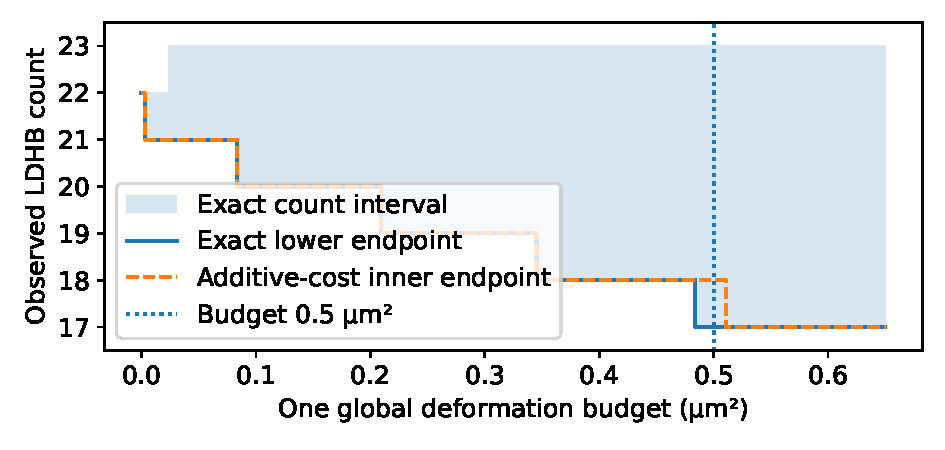
\includegraphics[width=.90\textwidth]{figures/count_curve.pdf}
\caption{The complete LDHB count-spectrum example under unchanged atlas geometry. Step changes follow exact rational minimum areas, rather than interpolation between sampled optimization outputs. The inner comparison can miss an attainable endpoint; the outer comparison can combine individually affordable but jointly over-budget changes.}
\end{figure}

\section{Alternative segmentation and interpretation limits}
Before evaluating outputs, a separate protocol specified the nearest labelled nuclear pixel within five physical micrometres as an image-only alternative reference. Pixels beyond that radius receive background label zero. Nuclear pixels carry the cell-mask owner. Transcript positions are unchanged. To avoid missing nuclei outside the crop, RNA within five micrometres of the crop edge is removed from \emph{both} reference count calculations. A gene is excluded if that removal intersects an editable part of its spectrum; all other unchanged and changed entries are retained.

\begin{table}[ht]\centering
\begin{tabular}{lrr}\toprule
Original-protocol count question&Lung&Breast format test\\\midrule
Included cell--gene entries&3,674&25,678\\
Different count from source&1,128&11,151\\
Changed count attainable at some atlas budget&185&1,818\\
Changed RNA assignments&1,094&15,578\\
Changes outside editable support&824&12,283\\
Locally infeasible requested patch assignments&56&494\\
Complete alternative vectors feasible&0/2&0/2\\\bottomrule
\end{tabular}
\caption{Original nuclear-reference protocol, before the shared-population refinement used in the width study. Countwise inclusion and joint-vector feasibility answer different questions; neither is accuracy against truth.}
\end{table}

A global increase in area cannot allow assignments excluded by fixed seams, candidate neighbors, nuclear constraints or bands. These exclusions are retained as infeasibility, not dropped during calibration. The analysis therefore reveals that this atlas cannot represent much of this particular alternative's disagreement. It is not a successful anatomical coverage study. Proseg was executed in the merged revision, as described below. The five-micrometre nuclear reference remains a distinct image-only alternative.

The three co-detection pairs are EPCAM/PTPRC, EPCAM/CD3D and EPCAM/PECAM1. The complete lung census contains 150 cell/pair questions at eight budgets; the breast census contains 1,148. Of seven lung source EPCAM/PTPRC positives, two become removable by budget 0.25. Of 48 breast source positives, two become removable. Other tested positives persist under the stated family. The vector spectra add no exclusion beyond marginal intervals on these inputs. Neither outcome determines whether co-detection is a real cell state, a doublet or leakage.

\section{Executed Proseg diagnostics and width sensitivity}
Proseg 3.2.0 was run on both existing lung crops. The default factorization failed on the first crop with an empty-input feature-selection error; this failure also occurred with an equivalent CSV input. Both completed runs disabled factorization, while retaining upstream sampling defaults: 200 burn-in iterations, 200 sampling iterations and 50 hill-climb steps, with two CPU threads. This adaptation was motivated by execution failure before comparing assignment results.

The first crop retained 5,774 of 5,847 supplied transcripts and returned 93 cells; the second retained 1,482 of 1,523 and returned 72 cells. Source-owner disagreements on retained IDs numbered 3,242 and 765, respectively. Proseg assigned 2,484 and 1,335 retained molecules to background. These large background fractions underline the limitations of sparse, clipped inputs. Single-run executable times were 14.14 and 10.67 seconds, excluding installation and adapters. Neither agreement nor disagreement establishes accuracy, and these timings give no whole-slide performance claim.

The raw output, exact commands, input/output hashes and excluded transcript identifiers are preserved. Proseg cell indices are mapped through original cell IDs. Reach questions use shared retained molecule IDs, original observed coordinates and identical source/alternative count populations. Molecules omitted from a scored population remain geometric constraints with zero score. The nuclear reference retains its own border guard. Comparison denominators therefore remain reference-specific.

\subsection{Declared width sensitivity protocol}
The post-review protocol was recorded before the width runs, after the earlier atlas analyses. It uses the same two lung crops from one donor and makes no claim of preregistration before the original results. The three proposed chart halfwidth caps are $B=4,12,28$, with fallback ladders $(4,2,1,1/2)$, $(12,4,2,1,1/2)$ and $(28,4,2,1,1/2)$. The candidate ordering, label containment checks, disjointness checks, source masks and nuclear constraints remain fixed. Each atlas is re-extracted and independently checked with exact rational geometry. Both greedy selection and the different ladders mean that these families are non-nested. In particular, the largest ladder omits the intermediate halfwidth 12.

The source transform gives $p=1048576/4934475\,\mu\mathrm m$ per pixel. The chart-to-physical displacement is $p|h|/\sqrt2$ and the band is $|h|\le3B/4$. Each accepted atlas contains a patch with the proposed halfwidth cap. The corresponding displacement caps are upper bounds before additional slope and nuclear restrictions, rather than optimized attainable or typical displacements: halfwidth 12 is accepted in 132 of 544 intermediate-cap patches and halfwidth 28 in 41 of 543 largest-cap patches; all other accepted halfwidths are at most 4. No physical scale is inferred from a nominal image resolution. Counts, patch acceptance and coverage are reported below.

\begin{table}[ht]\centering
\begin{tabular}{lrrr}\toprule
Chart halfwidth cap $B$&4&12&28\\\midrule
Largest band displacement cap ($\mu\mathrm m$)&0.451&1.352&3.155\\
Accepted patches / candidates&544/782&544/782&543/782\\
Editable incident boundary edges (\%)&68.300&67.907&68.058\\
Editable transcripts&745&1,288&1,220\\
Nuclear changed counts reachable&186/1,134&223/1,134&190/1,134\\
Proseg changed counts reachable&185/2,798&241/2,798&200/2,798\\\bottomrule
\end{tabular}
\caption{Reach at unlimited area on fixed shared-observation populations. Each count is tested separately by exact score-spectrum membership; full alternative count matrices need not be jointly attainable. The largest cap loses some reach because the re-extracted families are non-nested.}
\end{table}

The declared area budgets, in $\mu\mathrm m^2$, are $0$, $0.01$, $0.025$, $0.05$, $0.075$, $0.1$, $0.15$, $0.2$, $0.25$, $0.3$, $0.4$, $0.5$, $0.75$, $1$, $2$ and $4$. The exact count minima allow both evaluation on this grid and unlimited-area membership. At cap 4, nuclear reach attains its unlimited value by budget 0.25 and Proseg reach by 0.2. At cap 12, both reach their unlimited values by budget 2. At cap 28, budget 4 reaches 189 nuclear and 197 Proseg counts, compared with unlimited values of 190 and 200. No timed-out or failed solve is reported as a certificate. All study runs completed, and independent checks found zero failures among 8,270 local count/geometry witnesses and 25,610 global count/area traces.

\begin{figure}[ht]\centering
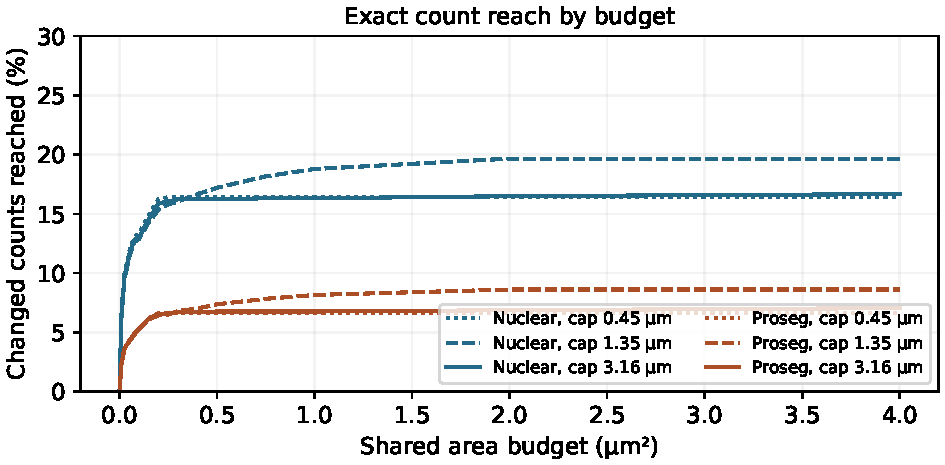
\includegraphics[width=.96\textwidth]{figures/reach_budget.pdf}
\caption{Exact reach as the shared area budget increases within each fixed width setting. Source and alternative counts use the same reference-specific retained molecule IDs. Curves from different width settings compare non-nested atlas families.}
\end{figure}

\subsection{Nuclear denominator audit}
The original nuclear comparison removed a gene whenever the five-micrometre crop-border guard intersected its editable spectrum. The width study scores only retained molecules, while keeping excluded molecules as zero-score geometric collateral. This permits six additional changed lung cell--gene questions in the default atlas. One, C7 in cell 153965, is reachable. Thus the refined default comparison is 186 of 1,134, compared with the original 185 of 1,128. Counts and reach agree for every previously shared question. The difference is an analysis-contract refinement, rather than an effect of increasing ribbon width. The audit preserves all six keys and their old/new inclusion status. The breast comparison retains the original protocol; it was not rerun across width settings.

The width study tests restricted geometric reach, rather than anatomical calibration. Each alternative count is assessed individually; reachable counts can still demand incompatible global assignments. Sparse clipped inputs, a single Proseg run per crop, adapted factorization and one lung donor limit interpretation. Source coordinates are held fixed, all transcript-ID exclusions are explicit, and agreement with an alternative segmenter supplies no ownership accuracy estimate.


\section{Validation and resource measurements}
The independent scalar reference uses Fraction arithmetic but imports none of the production implication, envelope, integrated-layer, min-cut or count-chain routines. It recomputes the minimum for every target assignment, then uses Cartesian products for global truth. Inputs and their extraction remain shared. Continuous witnesses have a further direct slope, band, owner, nuclear and rational-area check.

\begin{table}[ht]\centering
\begin{tabular}{lrr}\toprule
Check&Lung&Breast format test\\\midrule
Independent local gene spectra&706&7,068\\
Target binary assignments&1,498&17,542\\
Local witness records&1,101&11,594\\
Global spectra&3,304&22,976\\
Cartesian tuples&3,905&32,730\\
Global attaining count witnesses&3,876&29,799\\
Unique budget intervals&26,432&183,808\\
Exact half-ribbon/pixel checks&31,642&105,824\\
Relevant ribbon-pair checks&491&1,602\\
Nuclear pixel fragments&6,609&42,732\\\bottomrule
\end{tabular}
\caption{All checks completed without discrepancies. Counts are computational checks on repeated model inputs, not biological replicate counts.}
\end{table}

The merged entry point additionally checks atlas identity, source identity and the completed geometric audit before issuing a certificate; deliberate identity and structural alterations are rejected. The count-chain test suite additionally compares 201 scalar spectra on 100 generated systems, tests 80 nonflat models against 1,644 exhaustive assignments, verifies positive mandatory deformation and rejection of free interval-valued RNA, and checks the explicit eight-unit gap. All 944 multicopy local gene questions from both data collections agree with independently enumerated spectra. A full hybrid reanalysis uses the chain for all multicopy genes and closure for single-copy genes; every global minimum area and every interval CSV row matches the separately checked enumerated calculation. The transversely monotone gluing map passes inverse, trace, chart roundtrip and independent polygon-area checks.

\subsection{Count-chain scaling}
The fixed constructed family has flat source, slope one, equal flipped height $h=1/4$, site spacing $d=1/10$, clearance $1/1000$, a containing band and endpoints outside all tents. The minimum for $k\ge1$ changes is
\[
 A_k=h^2+(k-1)(hd-d^2/4),\qquad A_0=0,
\]
attained by $k$ consecutive sites. For arbitrary selected sites, each additional separation contributes at least the adjacent-site area increment, which proves the lower bound. This analytical family is a correctness/scaling test, not a difficult problem for every possible specialized algorithm.

\begin{table}[ht]\centering
\begin{tabular}{rrrrrr}\toprule
RNA&Count levels&Mesh nodes&Height candidates&Visited states&Median total(s)\\\midrule
16&17&111&1,154&8,112&0.465\\
32&33&207&2,370&35,104&1.574\\
64&65&399&4,802&147,456&7.138\\
128&129&783&9,666&605,632&42.206\\\bottomrule
\end{tabular}
\caption{Three fresh sequential processes per size. Total includes preparation, dynamic programming, all witness reconstruction and continuous checks. No limit is reached.}
\end{table}

The 128-RNA totals range from 40.189 to 42.704 seconds. Median mesh compilation is approximately 2.033 seconds and dynamic programming plus all witness output/checking approximately 40.152 seconds; separate medians need not sum exactly. The tested limits are 300,000 retained candidate heights, one million visited states, 60 seconds for preparation, 90 seconds for dynamic programming, and 160 seconds for a complete process. Requested single-thread environment variables are recorded, but the arithmetic is Python integer/Fraction work. Peak whole-process RSS at the largest size is approximately 205 MiB and includes imports. Raw process records contain the exact environment and wall/memory measurements.

\section{Reproduction, data rights and assistance}
The current package includes one command-line entry point, prepared rational atlases, original mask/transcript crops, complete interval and spectrum records, independent checkers, tests, manuscript sources and a checksum manifest. The exact prepared-input workflow uses the Python standard library. Raster extraction, source re-ingestion and the nuclear distance transform use the separately listed NumPy, pandas, SciPy, rasterio and shapely dependencies, with an optional PyArrow reader or the documented restricted Parquet fallback. Those dependencies are not silently required by the exact count solver.

The basic commands are:
\begin{verbatim}
python atlas_cli.py verify-manifest
python atlas_cli.py showcase --output run/showcase.json
python atlas_cli.py validate
python atlas_cli.py reproduce --dataset lung --output-dir run/lung
python atlas_cli.py reproduce --dataset breast --output-dir run/breast
\end{verbatim}
Scientific code is frozen at revision \href{https://github.com/arnavperam/geocert/tree/1cdbb9e0b4ea386c210fd231372900b2844dddba/atlas2027}{\nolinkurl{1cdbb9e0b4ea386c210fd231372900b2844dddba}}. The release record distinguishes new measurements from frozen-source replay. Merged source and results are available at \url{https://github.com/arnavperam/geocert/tree/atlas-merged-revision/atlas2027}. Software is MIT licensed; data retain their original 10x Genomics CC BY 4.0 attribution and breast test-use limitation. The AI-assistance disclosure accompanies the source. Computational cross-checks are not biological ground truth.
\end{document}
